\documentclass[11pt]{article}

\usepackage{graphicx}

% Enable references to labels in the notes
\usepackage{xr-hyper}
\externaldocument{p328_notes}
\usepackage{hyperref}

% Sans fonts
\usepackage{sfmath}
\renewcommand{\familydefault}{\sfdefault}

\newcommand{\COURSE}{PHYS328W}
\newcommand{\LABNUM}{6}
\newcommand{\TITLE}{Operational Amplifiers}
\markright{\COURSE~Lab \LABNUM\ : \TITLE}

\setlength{\textwidth} {6.5 true in}
\setlength{\textheight}{9 true in}
\setlength{\hoffset}   {-0.75 true in}
\setlength{\voffset}   {-0.75 true in}
\setlength{\parindent} {12 pt}
\pagestyle{myheadings}

\begin{document}

\thispagestyle{empty}

\section*{\COURSE\ Lab \LABNUM\ : \TITLE}

This assignment relies on Section~\ref{sec:opamps} of the notes.

\begin{figure}[ht]
  \begin{center}
    \scalebox{0.8}{
      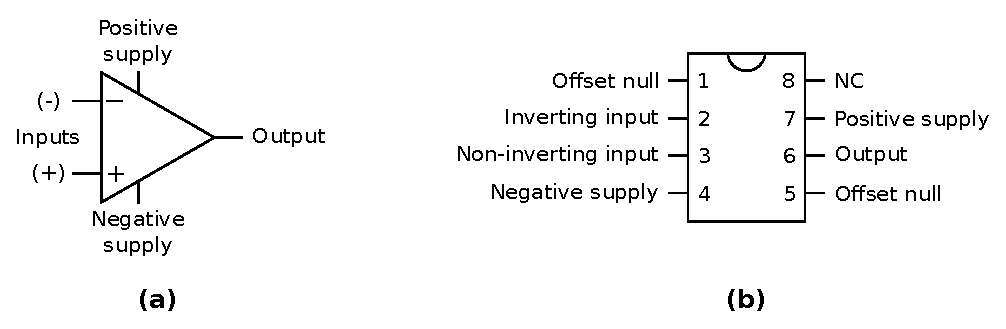
\includegraphics{opamp.eps}
    }
    \caption{(a) Schematic symbol of an operational amplifier, and
      (b) the connection diagram for the 8-pin dual inline package
      (DIP) of the \texttt{LM741} and \texttt{LF411} op amps.}
    \label{fig:opamp}
  \end{center}
\end{figure}

Amplifier circuits with nice properties --- high gain and 
high input impedance, for example --- packaged as integrated circuits
(ICs), are called \textbf{operational amplifiers} or op amps. They are
called ``operational'' amplifiers, because they can be used to perform
arithmetic operations like addition, subtraction, multiplication,
differentiation and integration with signals. The 
schematic symbol of an op amp is shown in Figure~\ref{fig:opamp} along
with the connection diagram for the \texttt{LM741} op amp we will use
here.

\begin{figure}[ht]
  \begin{center}
    \begin{tabular}{cc}
      \hspace{1cm}
      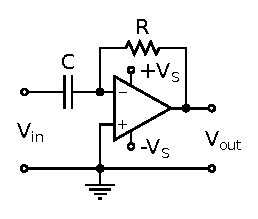
\includegraphics{differentiator.eps}
      \hspace{1cm}
      &
      \hspace{1cm}
      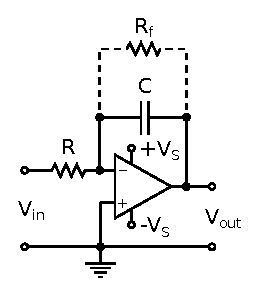
\includegraphics{integrator.eps}
      \hspace{1cm}
      \\
    \textbf{(a)} & \textbf{(b)}
    \end{tabular}
    \caption{(a) Schematic diagrams of (a) an op amp based
      differentiator circuit, and (b) an op amp based integrator
      circuit.}
    \label{fig:diffint}
  \end{center}
\end{figure}

In this lab, you will simulate, build, and investigate either the
differentiator or the integrator circuit shown in
Figure~\ref{fig:diffint}. Our strategy for this lab is to use
simulations to guide the design.

\subsection*{Simulations}

Choose either the differentiator circuit
(Section~\ref{sec:differentiator} of the notes) or the integrator
circuit (Section~\ref{sec:integrator} of the notes).

\begin{enumerate}
\item Starting with $R = 1$~k$\Omega$, make educated guesses at values
  for $C$ and $R_f$. 
  
\item Construct the circuit shown in Figure~\ref{fig:diffint}(a)
  or \ref{fig:diffint}(b). For the op amp, click on
  \texttt{Place -> Part ...}, type LM741 into the search bar, and
  select \texttt{LM741/OPAMP}.

  If the part does not show up in the \texttt{Part List} panel, you
  need to add a library. Click the \includegraphics{OrCAD_AddLib.png}
  button in the \texttt{Libraries} panel, select the file
  \texttt{opamp.olb}, and click \texttt{Open}. Then, select the
  \texttt{OPAMP} library in the \texttt{Libraries} panel, and try
  searching for \texttt{LM741/OPAMP} again.
  
  If you do not see a list of libraries (\texttt{.olb} files) when you
  click the \includegraphics{OrCAD_AddLib.png} button, use the file
  browser to navigate to:
  \begin{quote}
    \verb+C:\Cadence\SPB_17.2\tools\capture\library\pspice+
  \end{quote}

\item Use a Pulse voltage source to define a 1~kHz triangle wave for
  the differentiator, or a 1~kHz square wave for the integrator, with
  a 1~V amplitude. The parameters of the pulse source are
    \begin{center}
      \begin{tabular}{ll}
        \texttt{V1}  & Low voltage \\
        \texttt{V2}  & High voltage \\
        \texttt{TR}  & Rise time from $V_1$ to $V_2$ \\
        \texttt{PW}  & Time at $V_2$ \\
        \texttt{TF}  & Fall time from $V_2$ to $V_1$ \\
        \texttt{PER} & Period \\
        \texttt{TD}  & Delay (shifts the entire waveform)
      \end{tabular}
    \end{center}

\item Place voltage probes in the schematic to measure $V_{in}$ and
  $V_{out}$.
  
\item Define a transient simulation profile and adjust the values of
  $R_f$ and $C$ as needed to give acceptable output (either the
  derivative or the integral of the input signal).

\end{enumerate}

\subsection*{Experiments}
\begin{enumerate}
\item Build the circuit you designed with the help of your
  simulations. (Choose actual component values as close to your
  simulated ones as possible.)

\item Use a function generator to drive your circuit with either a
  1~kHz triangle wave (differentiator) or a 1~kHz square wave
  (integrator) with a 1~V amplitude.

\item Figure out how to export a screen capture the measured $V_{out},
  V_{in}$ vs. time display from your oscilloscope for your report.

\item Determine empirically the frequency range over which the circuit
  produces acceptable output.
  
\item Run a final simulation using the measured values of the actual
  components you used and produce a simulated $V_{out}, V_{in}$
  vs. time graph (at 1~kHz) for your report.
  
\end{enumerate}

\subsection*{Products}

Upload to Canvas a brief \LaTeX\ report in which you describe ...
\begin{itemize}
\item your design process (simulations).

\item the level of agreement between your simulated and measured
  $V_{out}, V_{in}$  vs. time graphs. 

\item the level of agreement between the simulated and empirical
  frequency ranges within which your circuit produced acceptable
  output.
  
\end{itemize}
Include as figures the schematic of your final circuit and your
measured and simulated $V_{out}, V_{in}$ vs. time graphs.

\end{document}
